\section{System modeling}

\subsection{Energy-Flow description}

A system can be modeled as sub-modules that are connected through energy ports with \textit{effort} $e$ and \textit{flow} $f$. In order to preserve causality, each sub-module has either all flow going in to it, or all effort going in to it. 

\begin{figure}[H]
    \centering
    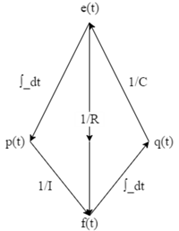
\includegraphics{figures/effort-flow.png}
    \caption{Relation between effort, flow, momentum and displacement}
    \label{fig:relation_effort_flow}
\end{figure}
\begin{figure}[H]
    \centering
    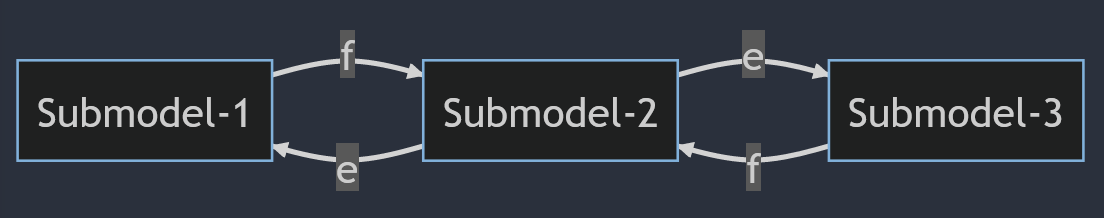
\includegraphics[scale=0.5]{figures/effort-flow-submodules.png}
    \caption{Submodules}
    \label{fig:effort-flow-submodules}
\end{figure}

\begin{table}[H]
    \centering
    \begin{tabular}{|m{6em}|c|m{12em}|m{14em}|}
        \hline
        Term    & Symbol    & Description   & Equation 
        \\\hline
        Flow    & $f$       & Time derivative of displacement & 
        \\\hline
        Effort  & $e$       & The energy per unit of displacement & 
        \\\hline
        Displacement    & $q$   & A quality related to static behavior  & $q(t)=\int f(t)dt$
        \\\hline
        Power&	P&	Time integral of effort	& $P=f^\top(t)e(t)$
        \\\hline
        Inertance (Inertia)	& I	& Momentum storage element	& $e=\frac{d}{dt}(If)=\frac{d}{dt}(f)I+\frac{d}{dt}(f)I$
        \\\hline
        Dissipation/ Resistance & R & Power dissipative element	& $f(t)=\frac{1}{R}e(t)$
        \\\hline
        Compliance	& C	& Charge storage element &	$e(t)=\frac{1}{C}q(t)$
        \\\hline
        Momentum &	p &	Time integral of effort &	$\dot{p}=e$
        \\\hline
        Energy	& E	& Conserved quantity in closed systems& 	$q^\top(t)e(t)$
        \\\hline
    \end{tabular}
    \caption{Energy flow in different domains}
    \label{tab:my_label}
\end{table}

\subsection{Energy-Flow in different domains}

\begin{table}[h]
    \centering
    \tiny
    \begin{tabular}{|m{5em}|m{5em}|m{5em}|m{5em}|m{6em}|m{5em}|m{6em}|m{6em}|}
        \hline
        \textbf{Domain} & \textbf{Effort} $e$ &	\textbf{Flow} $f$ &	\textbf{Inertance} $I$ & \textbf{Momentum} $p$	& \textbf{Resistance} $R$	& \textbf{Displacement} $q$	& \textbf{Compliance} $C$ 
        \\\hline
        Linear Mechanics	& Force $F$	& Velocity $v$	& Mass $m$	& Linear momentum $p$	& Damper $d$ in $F=d\dot{x}$	& Displacement $x$	& Inverse spring constant $1/k$ 
        \\\hline
        Angular Mechanics	& Torque $T$	& Angular velocity $\omega$	& Moment of inertia $J$	& Angular momentum $h$	& Angular damping ^^	& Angular displacement $\theta$	& Inverse angular spring constant 
        \\\hline
        Hydraulics	& Pressure $p$	& Volume flow $Q$	& Inertance $I$	& Hydraulic momentum $\pi$	& 	& 	&  
        \\\hline
        Electrical	& Voltage $v$	& Current $i$	& Inductance $L$	& Magnetic flux $\lambda$	& Resistance $R$	& Charge $C$	& Capacitance $C$ 
        \\\hline
        Thermal	& Enthalpy 	& Mass flow $m$ 	& Volume $V$ & & & &
        \\\hline
    \end{tabular}
    \caption{Energy flow in different domains}
    \label{tab:energyDomain}
\end{table}



\subsection{Power Transformations}
\textbf{Power conservative transformations}

We relate the efforts on both ports
\begin{equation}
    \begin{split}
        P_1&=P_2\\
        e_1f_1&=e_2f_2
    \end{split} 
\end{equation}

\textbf{Gyration:}

We relate the flow on one port to the effort on the other with a constant $g$
\begin{equation}
    \begin{split}
        e_2&=gf_1\\
        e_1&=gf_2
    \end{split}
\end{equation}

\subsection{Actuator Dynamics}
\subsubsection{Electrical Motors}
A motor shaft that rotates with $\omega_m$ has the equation of motion
$$J_m\dot{\omega}_m=T-T_L$$ where $T_L$ is the load torque acting on the shaft and $T$ is the motor torque.

The mechanical power is given by
$$P_m = T\omega_m \qquad P_L = T_L\omega_m$$

\subsubsection{Gear Model}
A gear with gear ratio $n$ may be described as
$$\omega_{out}=n\omega_{in}$$
$$T_{out} = \frac{1}{n} T_{in}$$

\subsubsection{Motor and Gear}
The equations of motion for motor, gear and load referred to the load side is
$$(\frac{1}{n^2}J_m + J_L)\dot{\omega}_m = \frac{1}{n}T - T_e$$

where $T_e$ is an external torque that acts on the load. 

The equations of motion for motor, gear and load referred to the motor side is
$$(J_m + n^2J_L)\dot{\omega}_m = T - nT_e$$
\subsubsection{Transformation of rotation to translation}
A rotation to translation transmission can be described by 
$$v=r\omega_m
\qquad F=\frac{1}{r}T_L$$
where $r$ is the radius.

This gives the equations of motion for motor and load referred to the load side is
$$(\frac{1}{r^2}J_m + m)\dot{v} = \frac{1}{r}T - F_e$$

where $T_e$ is an external force that acts on the load. 

The equations of motion for motor, gear and load referred to the motor side is
$$(J_m + mr^2)\dot{\omega}_m = T - rF_e$$

\subsubsection{Diesel Engine Model}

How the engine is modelled is based on the fidelity of the model (how close to reality),

\begin{itemize}
    \item High: 3D models of gas, crank shaft.
    \item Mid: Rate-limit, mechanical and thermal losses.
    \item Low: Applied torque with torque/power saturation.
\end{itemize}

In this course, we look at the low fidelity model with some elements of the energy loss.

Torque/power equation,

$$
\begin{aligned}
    P &= T \cdot \omega \Rightarrow P_{\text{max}}(\omega) = T_{\max} \cdot \omega
    \\
    T_{\max} &= \frac{P_{\max}(\omega)}{\omega}
    \\
    u &= \text{Needed torque}
    \\
    T_\text{sat} &= \min(u,T_{\max}(\omega))
    \\
    J_E\dot{\omega} - R_E\omega &= T_{\text{sat}} - T_{\text{load}}
\end{aligned}
$$

Where $E$ subscript signifies "engine". The two bottom formula gives either $\omega$ or $T$ based on what we need. \textbf{Add compliance to the model if necessary}.

\subsubsection{Electrical Actuators}

In this course, we look at DC-motors with constant field.

The model contains,

\begin{itemize}
    \item Voltage source, $u_a$
    \item Current, $i_a$
    \item Armature resistance, $r_a$
    \item Armature inductance, $L_a$
    \item Motor shaft properties, $\omega_m, T_m, J_m$
    \item Armature voltage, $e_a$
\end{itemize}

\begin{align}
    \begin{split}
        J_m \Dot{\omega}_m &= T - T_L
        \\
        T &= K_T i_a
        \\
        e_a \cdot i_a &= T \omega_m = K_T \omega_m
    \end{split}
\end{align}

$K_T$ is a proportional constant which is based on motor properties.

We have "inertance",

\begin{align}
    \begin{split}
        L_a \frac{d}{dt}(i_a) &= \sum u
        \\
        &= -R_ai_a - e_a + u_a
        \\
        &= -R_ai_a - K_T \omega m + u_a
        \\
        J_m\Dot{\omega}_m &= K_Ti_a - T_L
    \end{split}
\end{align}

The first and last equations is now our state space for DC-motor.

The control system can be modelled as such,

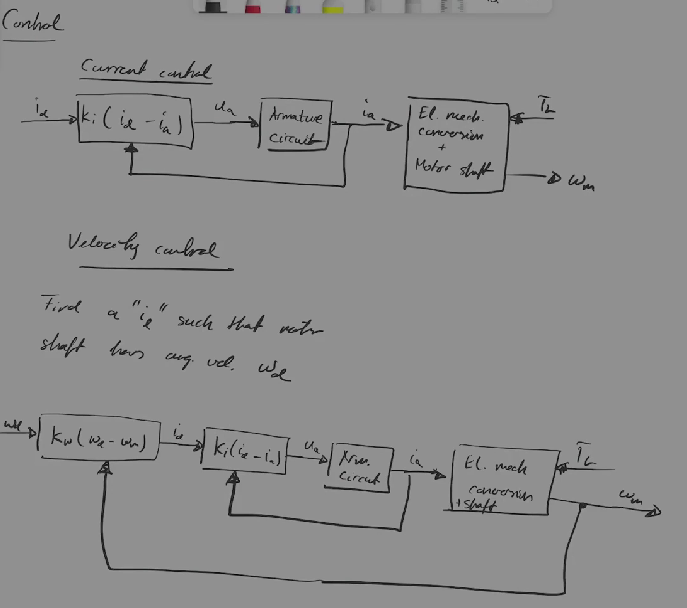
\includegraphics[width=12cm]{figures/DCMotor_MODSIM.png}

\subsubsection{Hydraulic Systems}

The reynolds number for fluid through pipe is calculated,

\begin{equation}
    Re = \frac{D}{A\cdot\gamma} \cdot Q
\end{equation}

where,

\begin{itemize}
    \item Diameter of tube: $D$
    \item Cross section area: $A$
    \item Viscocity of fluid: $\gamma$
    \item Flow rate: $Q$
\end{itemize}

If $Re > 1000$ we have turbulent flow, or if $Re < 10$ we have laminar flow. This is important as the flow rate $Q$ through a valve has different models based on type of flow,

\begin{align*}
    \begin{split}
        Q_l &= C_l \cdot \Delta P
        \\
        Q_T &= C_d A \sqrt{\frac{2}{\rho}\Delta P}
    \end{split}
\end{align*}

where,

\begin{itemize}
    \item Laminar and turbulent flow rate: $Q_l \& Q_T$
    \item Constants: $C_l \& C_d$
    \item Pressure difference over valve: $\Delta p$
    \item Cross section area: $A$
    \item Density of fluid: $\rho$
\end{itemize}

A good method for the model would be to switch between laminar and turbulent formula based on a guard (said not to appear on exam). Calculation on a 4-way valve can be seen in Figure \ref{fig:4wayvalve}.

\begin{figure}[H]
    \centering
    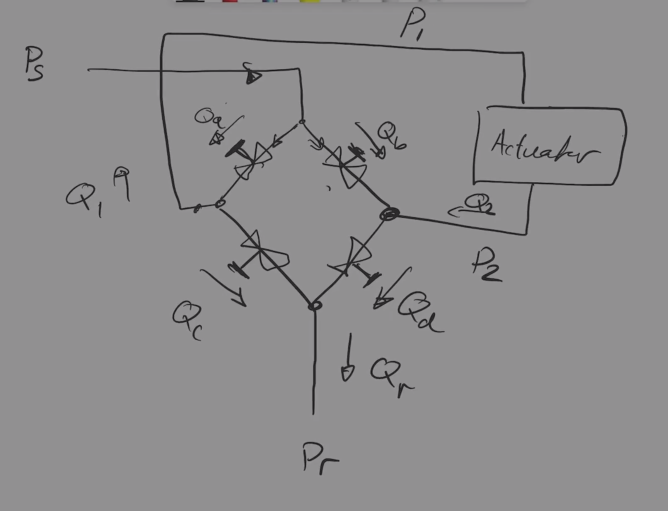
\includegraphics[width=6cm]{figures/4WayValve_MODSIM.png}
    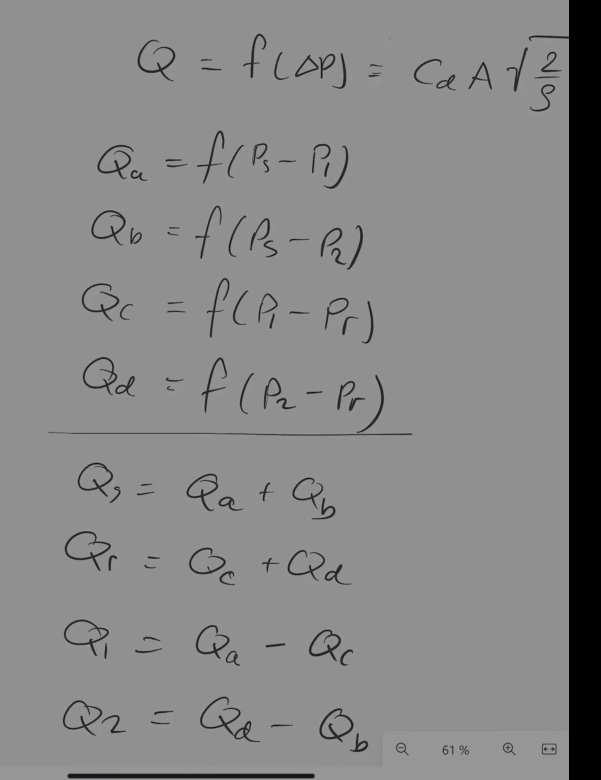
\includegraphics[width=6cm]{figures/4WayValveVar_MODSIM.png}
    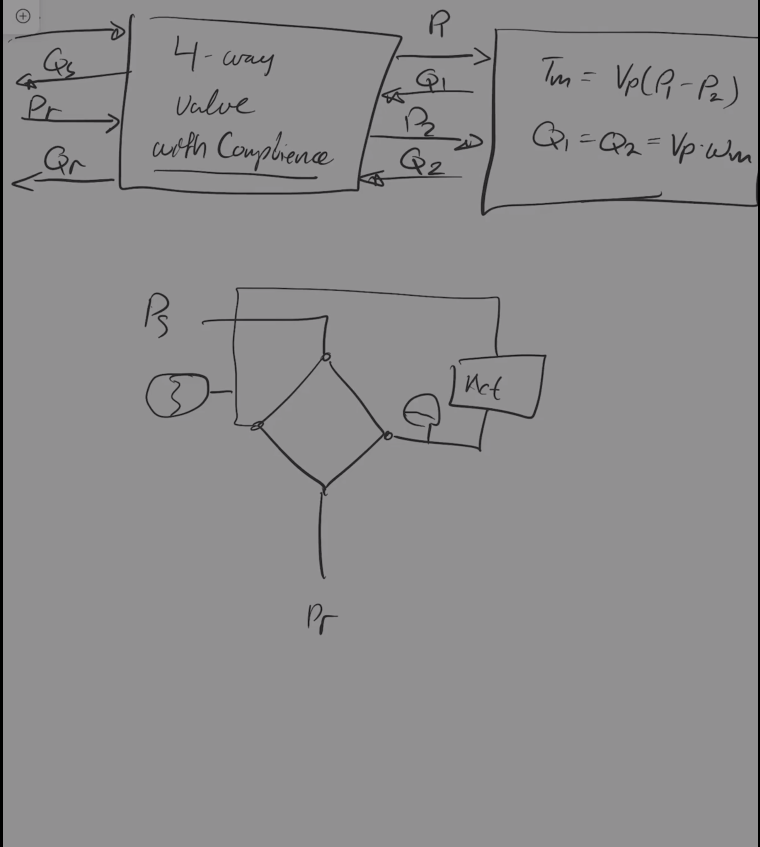
\includegraphics[width=6cm]{figures/4WayValveEndMe_MODSIM.png}
    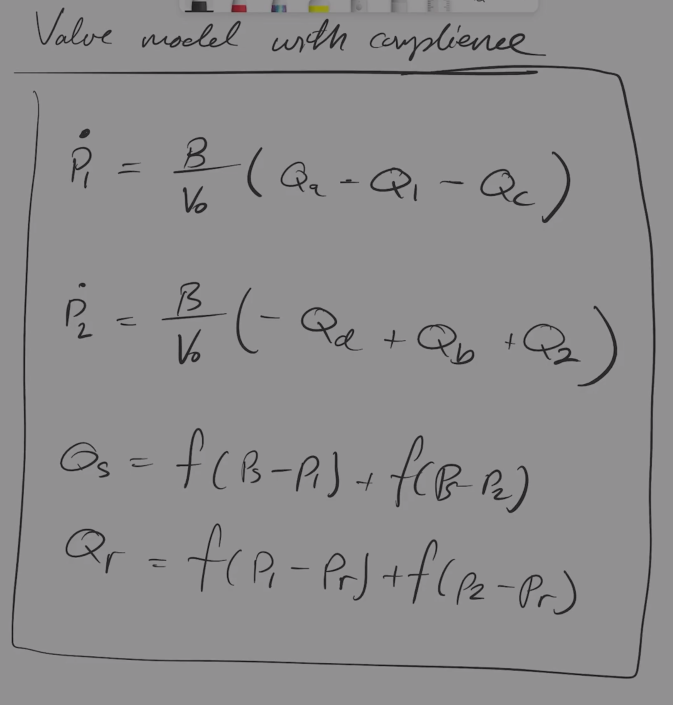
\includegraphics[width=6cm]{figures/4WayValveCompliance_MODSIM.png}
    \caption{4-way valve stuff.}
    \label{fig:4wayvalve}
\end{figure}

\subsection{Linear actuator}

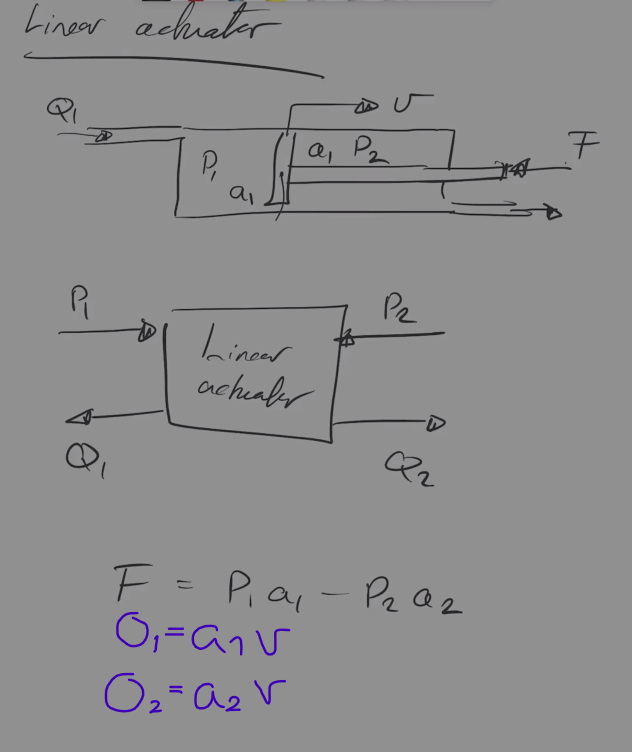
\includegraphics[width=6cm]{figures/linearactuator_MODSIM.png}

\subsection{Friction}
Linear friction is a force/torque proportional to the velocity $v$ or angular velocity $\omega$ by friction constant $R$. The force always points in the opposite direction of the movement.
$$
F=-Rv, \text{ or } T=-R\omega
$$

\subsection{Compliance}

Elastic shaft equations: 

\begin{equation}
\begin{aligned}
    \Delta \omega = \omega_m - \omega_1 \\
    \Delta \dot\theta  = \omega_m - \omega_1 \\
    T_L = K\Delta\theta + D\Delta\omega \\
    T_1 = T_L
\end{aligned}
\end{equation}

One can probably choose to use or not to use $D\neq0$. Book uses $D\neq0$, actuator lectures use $D=0$.

This is based on a book example, see figures \ref{fig:model_network} and \ref{fig:model_network_equations}.
\begin{figure}[H]
    \centering
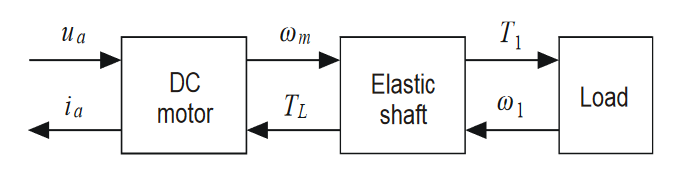
\includegraphics[width=0.7\textwidth]{figures/model_network.PNG}
    \caption{}
    \label{fig:model_network}
\end{figure}

\begin{figure}[H]
    \centering
    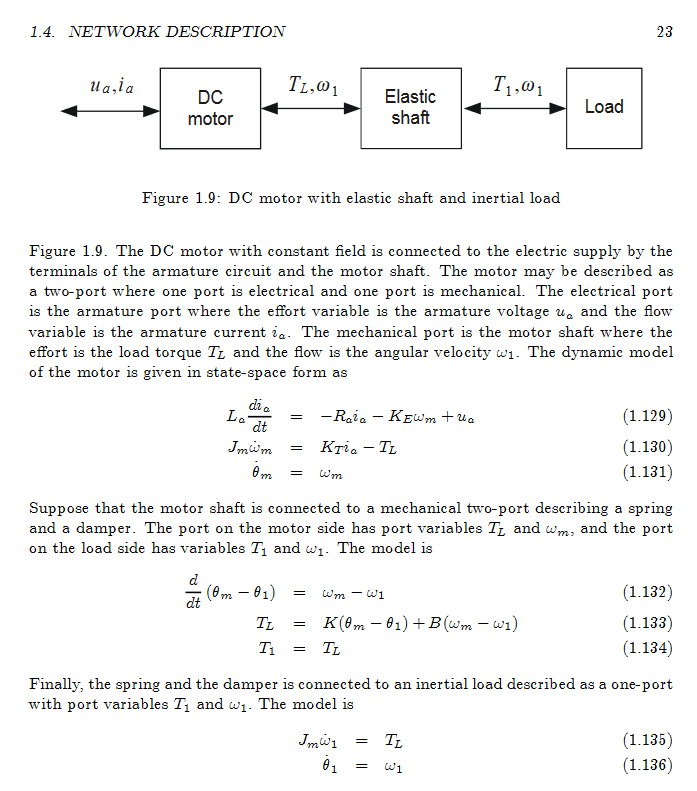
\includegraphics{figures/model_network_equations.PNG}
    \caption{Caption}
    \label{fig:model_network_equations}
\end{figure}